\documentclass{beamer}
\usetheme[block=fill, subsectionpage=progressbar]{metropolis}
\setbeameroption{show notes on second screen=right}

\title{Design and Analysis of 2x2 Cross-Over Trials with Continuous Data}
\author{Jules Lanari-Collard}
\institute{McGill University}
\date{August 23, 2024}

\usepackage{booktabs}

\begin{document}

\frame{\titlepage}

\section{Introduction to Cross-Over Trials}
\begin{frame}{The Cross-Over Design}
\begin{definition}
    A cross-over trial is a ``trial in which subjects are given sequences of treatments with the object of studying differences between individual treatments” \cite{senn2002crossover}.
\end{definition}
\note[item]{Differs from PGT, where subjects only receive 1 treatment.}
\note[item]{Most common design is 2x2 - AB/BA example.}
\note[item]{Either 2 active treatments, or 1 active and 1 control}
\note[item]{Typically used for chronic diseases - no question of curing underlying problem. e.g. athsma, rheumatism, epilepsy, migranes.}
\end{frame}

\begin{frame}{Randomisation}
    Only the \textit{order} of treatments is randomised:
    \begin{itemize}
        \item Validity of treatment comparison does not depend on randomisation.
        \item Randomisation does not guarantee unbiased comparison of treatments.
        \item Treatment groups differ with respect to their recent exposure to potentially effective treatments.
    \end{itemize}
    
    \begin{alertblock}{Fundamental Issue of Cross-Over Design}
        The comparability of treatments is not guaranteed by the structure of the trial alone, but instead depends on the treatments themselves \cite{piantadosi2005clinical}.
    \end{alertblock}
\end{frame}

\begin{frame}{Advantages}
    \begin{itemize}
        \item More observations per treatment \cite{senn2002crossover}
        \item Data in terms of \textit{difference to control}
        \item Improved recruitment rates
        \item Reduced spill-over rates \cite{piantadosi2005clinical}
    \end{itemize}
    \note[item]{Significant resource savings}
    \note[item]{Difference to control: eliminates between-patient variation (> within-patient variation)}
    \note[item]{Within-subject responses are positively correlated, reducing variance in treatment difference from control.}
    \note[item]{Improved recruitment - everyone guaranteed to receive both treatments.}
    \note[item]{Spillover - if treatment known to be desirable (e.g. exercise)}
\end{frame}

\begin{frame}{Disadvantages}
    \begin{itemize}
        \item Longer/inconvenient for subjects
        \item Complex analysis
        \item Cannot be used for infectious diseases
        \item Risk of drop-out
        \item Period-by-treatment interactions
    \end{itemize}
    \note[item]{Drop-out - all observations required for analysis of cross-over. PGT can recover information}
    \note[item]{Period-by-treatment interaction - effect of treatment not constant over time.}
\end{frame}

\begin{frame}{Carryover}
    \begin{definition}
        Carryover is the persistence of a treatment applied in one period in a subsequent period of treatment \cite{senn2002crossover}.
    \end{definition}
    \begin{itemize}
        \item Introduces bias to direct treatment effect estimates.
        \item Difficult to test and adjust for.
        \item Best solution is to introduce a wash-out period \cite{senn2002crossover}.
    \end{itemize}
    \note[item]{Patient not in state they would have been in without treatment in 1st period.}
    \note[item]{Effect of one treatment misinterpreted as effect of both treatments combined.}
    \note[item]{Models require additional assumptions, tests difficult to interpret independently of TE.}
    \note[item]{Wash-out period: period allowing effects of previous treatment to disappear.}
    \note[item]{Consequence - all conclusions are conditional on absence of carryover effect.}
\end{frame}

\section{Summary and Visualisation of Cross-Over Trial Data}

\begin{frame}{COPD Trial}
    \begin{itemize}
        \item 2x2 cross-over design.
        \item Comparing effectiveness of an inhaled drug A against a placebo (B).
        \item Treatment administered twice daily to patients with chronic obstructive pulmonary disease (COPD).
        \item 66 patients randomised into either AB or BA sequence (complete data obtained on 56).
        \item Outcome measurement is \textit{peak expiratory flow rate} (PEFR), measured 3 times per day (recording highest value).
    \end{itemize}
\end{frame}

\begin{frame}{Sample Data}
    \begin{table}

\caption{\label{tab:pefrDataSubsample}Subsample of COPD Trial Data (PEFR in L/min)}
\centering
\begin{tabular}[t]{lllrr}
\toprule
Sequence & Subject & Subject Label & Period 1 & Period 2\\
\midrule
AB & 1 & 7 & 121.90 & 116.67\\
AB & 2 & 8 & 218.50 & 200.50\\
AB & 3 & 9 & 235.00 & 217.14\\
AB & 4 & 13 & 250.00 & 196.43\\
AB & 5 & 14 & 186.19 & 185.50\\
\bottomrule
\end{tabular}
\end{table}

\end{frame}

\begin{frame}{Summary Table}
    \begin{table}

\caption{\label{tab:pefrDataSummary}Summary Table for PEFR Data}
\centering
\begin{tabular}[t]{l>{}r|rrrrrr}
\toprule
\multicolumn{2}{c}{ } & \multicolumn{2}{c}{Overall} & \multicolumn{2}{c}{Period 1} & \multicolumn{2}{c}{Period 2} \\
\cmidrule(l{3pt}r{3pt}){3-4} \cmidrule(l{3pt}r{3pt}){5-6} \cmidrule(l{3pt}r{3pt}){7-8}
 &  & Mean & SD & Mean & SD & Mean & SD\\
\midrule
AB & 27 & 242.52 & 81.53 & 245.84 & 82.78 & 239.20 & 81.70\\
BA & 29 & 223.08 & 72.99 & 215.99 & 72.63 & 230.16 & 73.94\\
\midrule\\
Total & 56 & 232.45 & 77.49 & 230.38 & 78.43 & 234.52 & 77.20\\
\bottomrule
\end{tabular}
\end{table}

    \note[item]{Normal data: mean/SD, otherwise median/IQR}
\end{frame}

\subsection{Summary Plots}

\begin{frame}{Boxplot}
    \begin{figure}
    \centering
    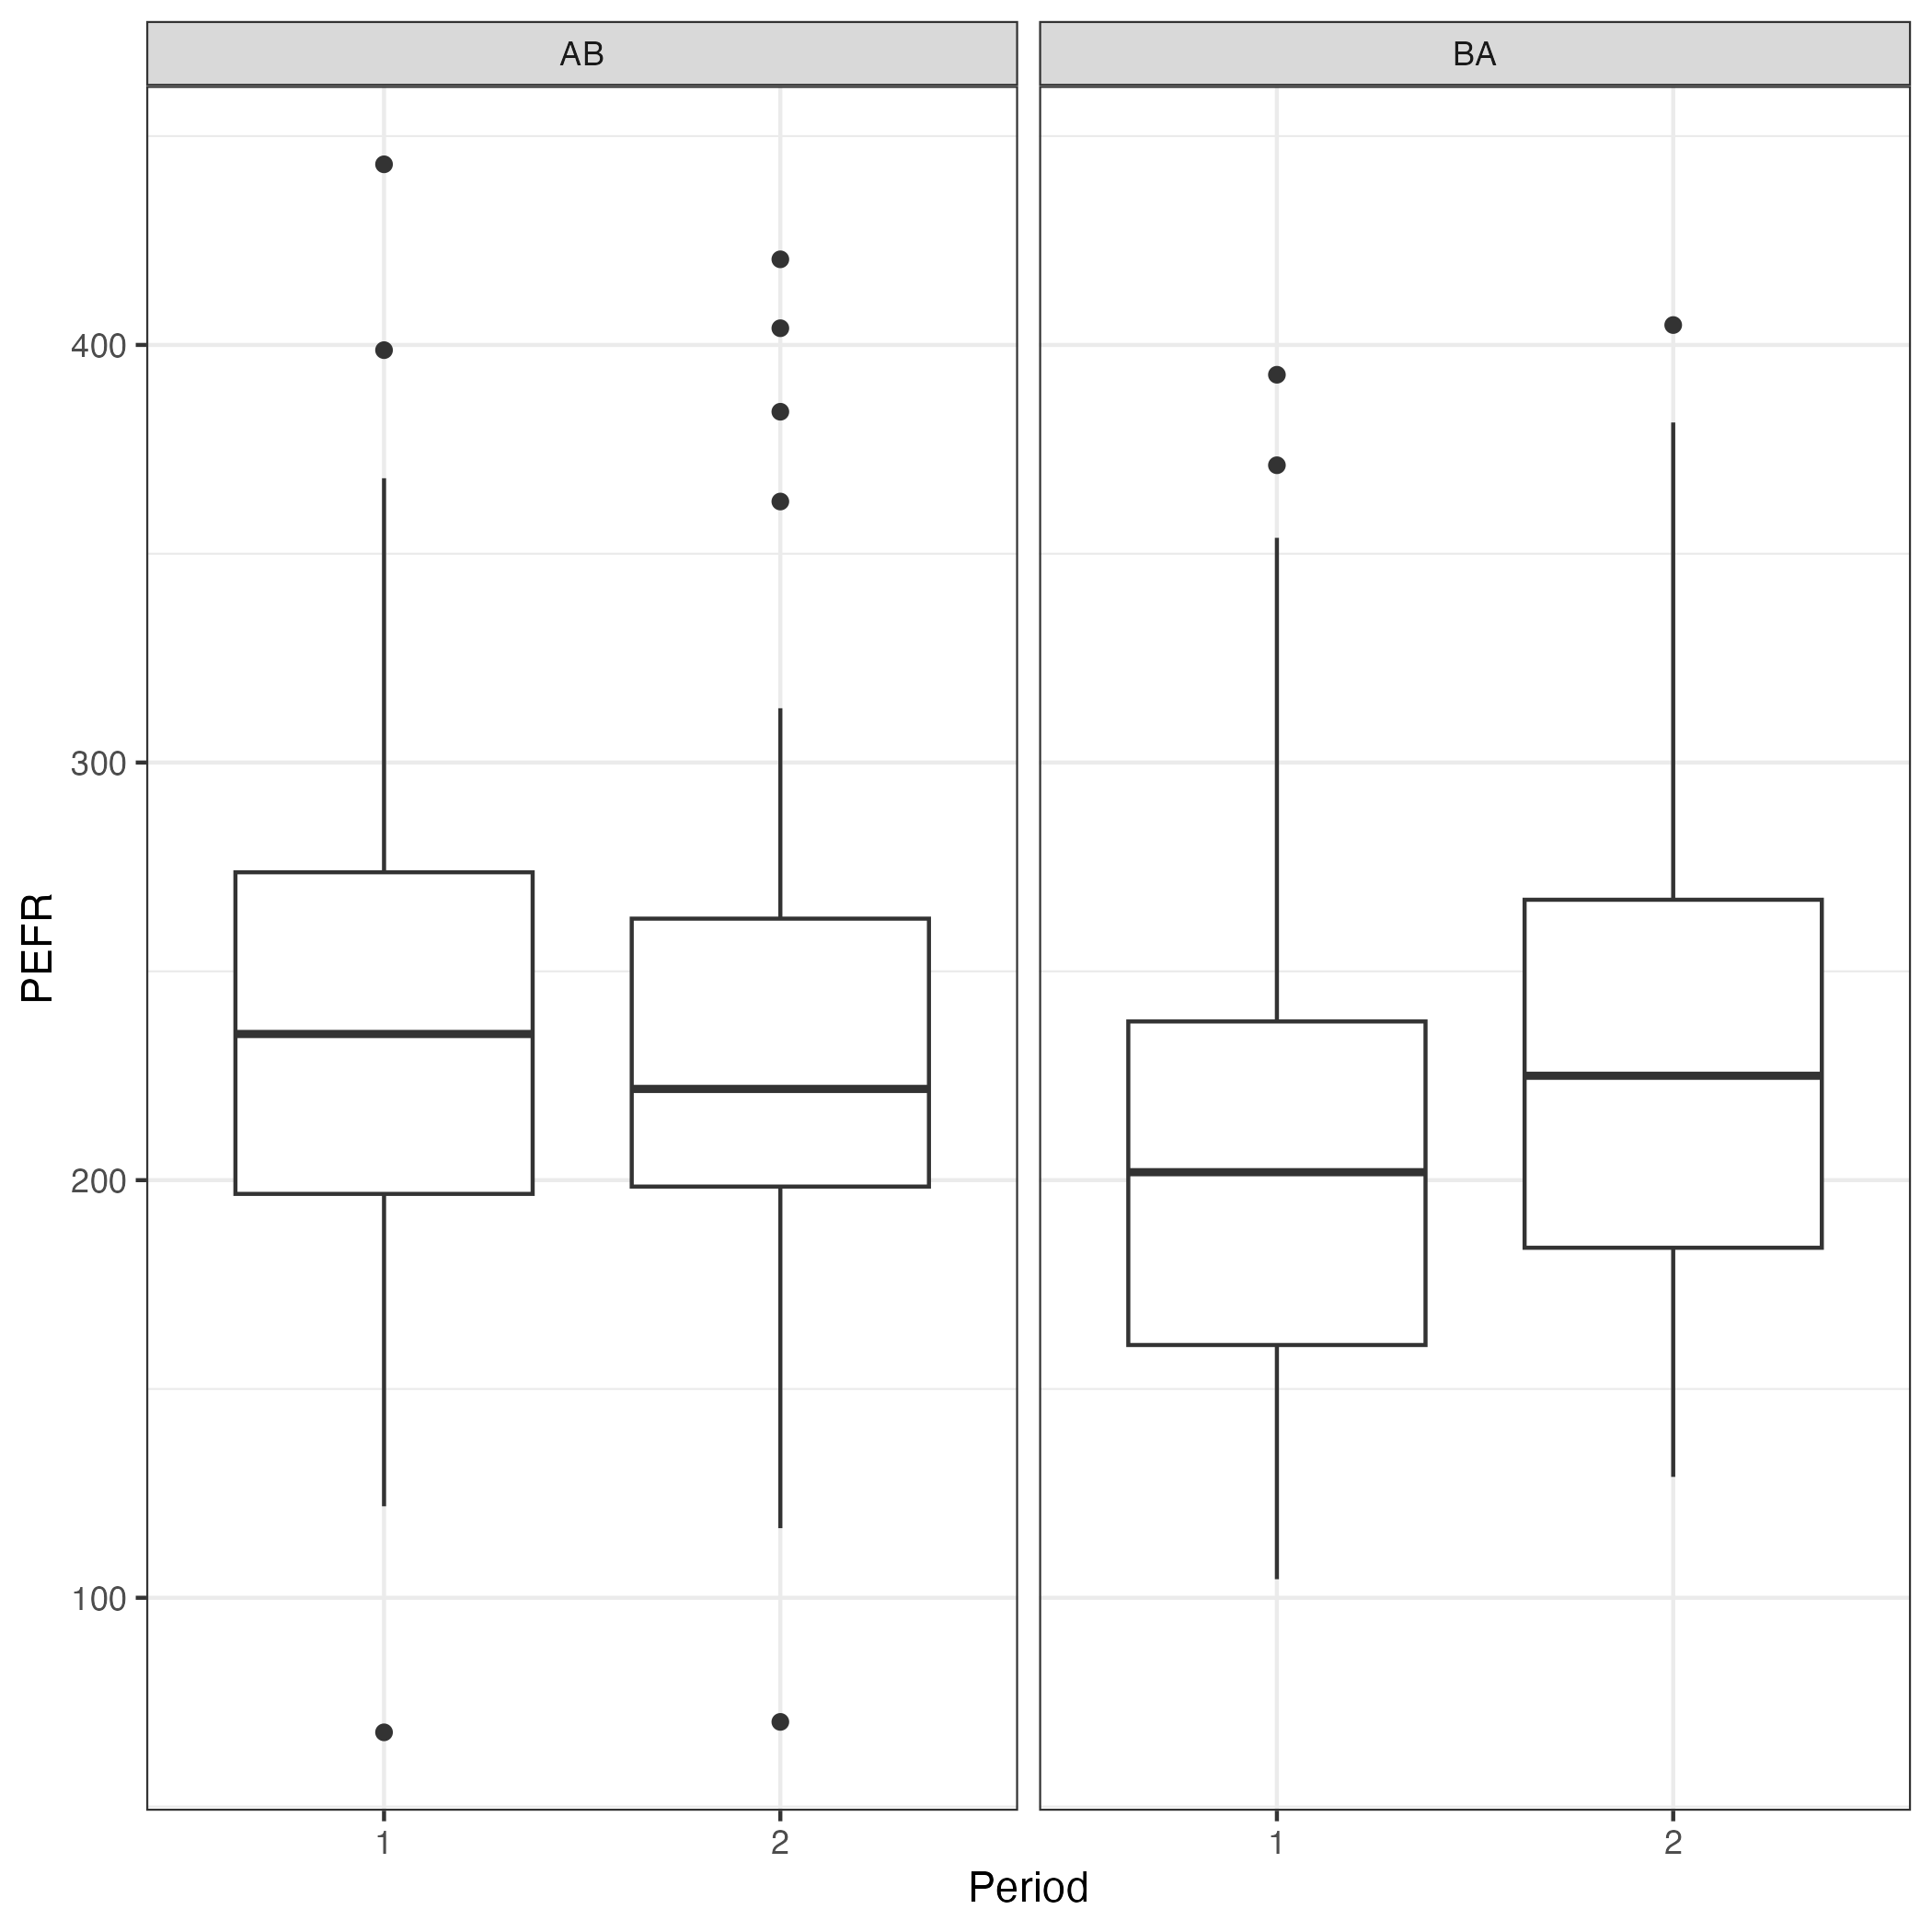
\includegraphics[width=\linewidth]{report/figures/ch2/boxplot.png}
\end{figure}
\end{frame}

\begin{frame}{Subject-Profiles Plot}
    \begin{figure}
        \centering
        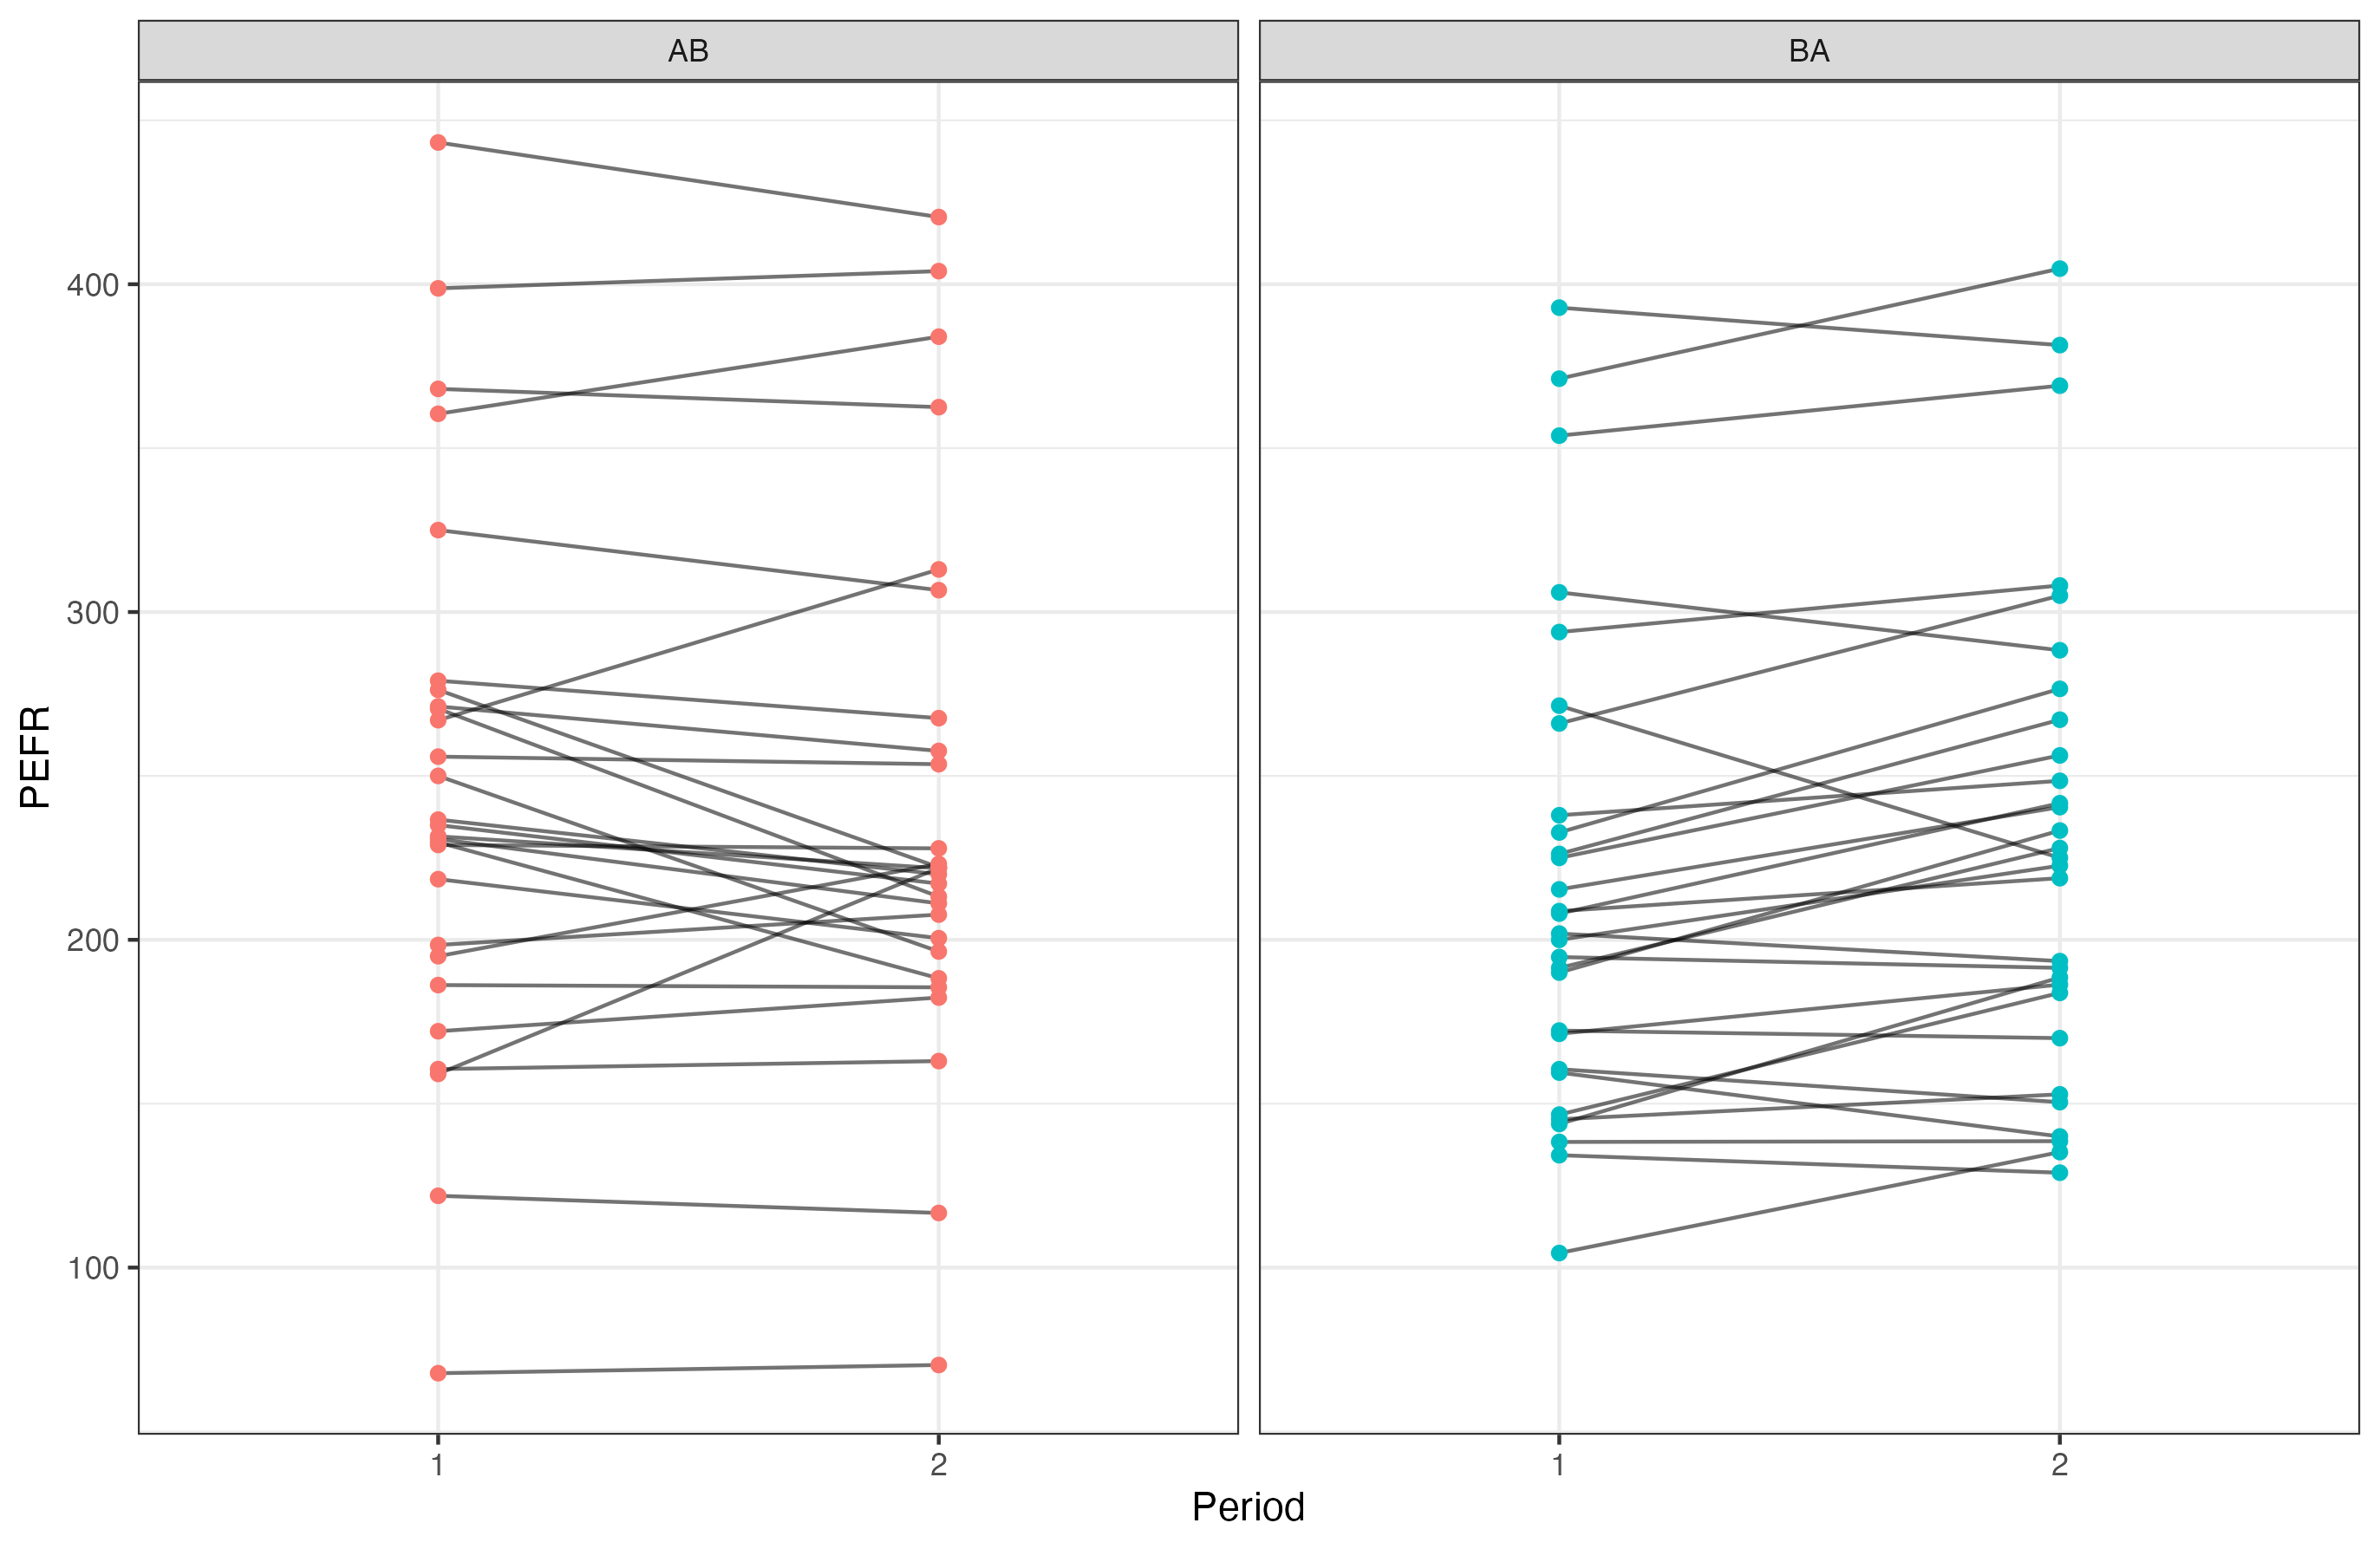
\includegraphics[width=\linewidth]{report/figures/ch2/subjectProfilesPlot.png}
    \end{figure}
\end{frame}

\begin{frame}{Period 2 vs Period 1}
    \begin{figure}
        \centering
        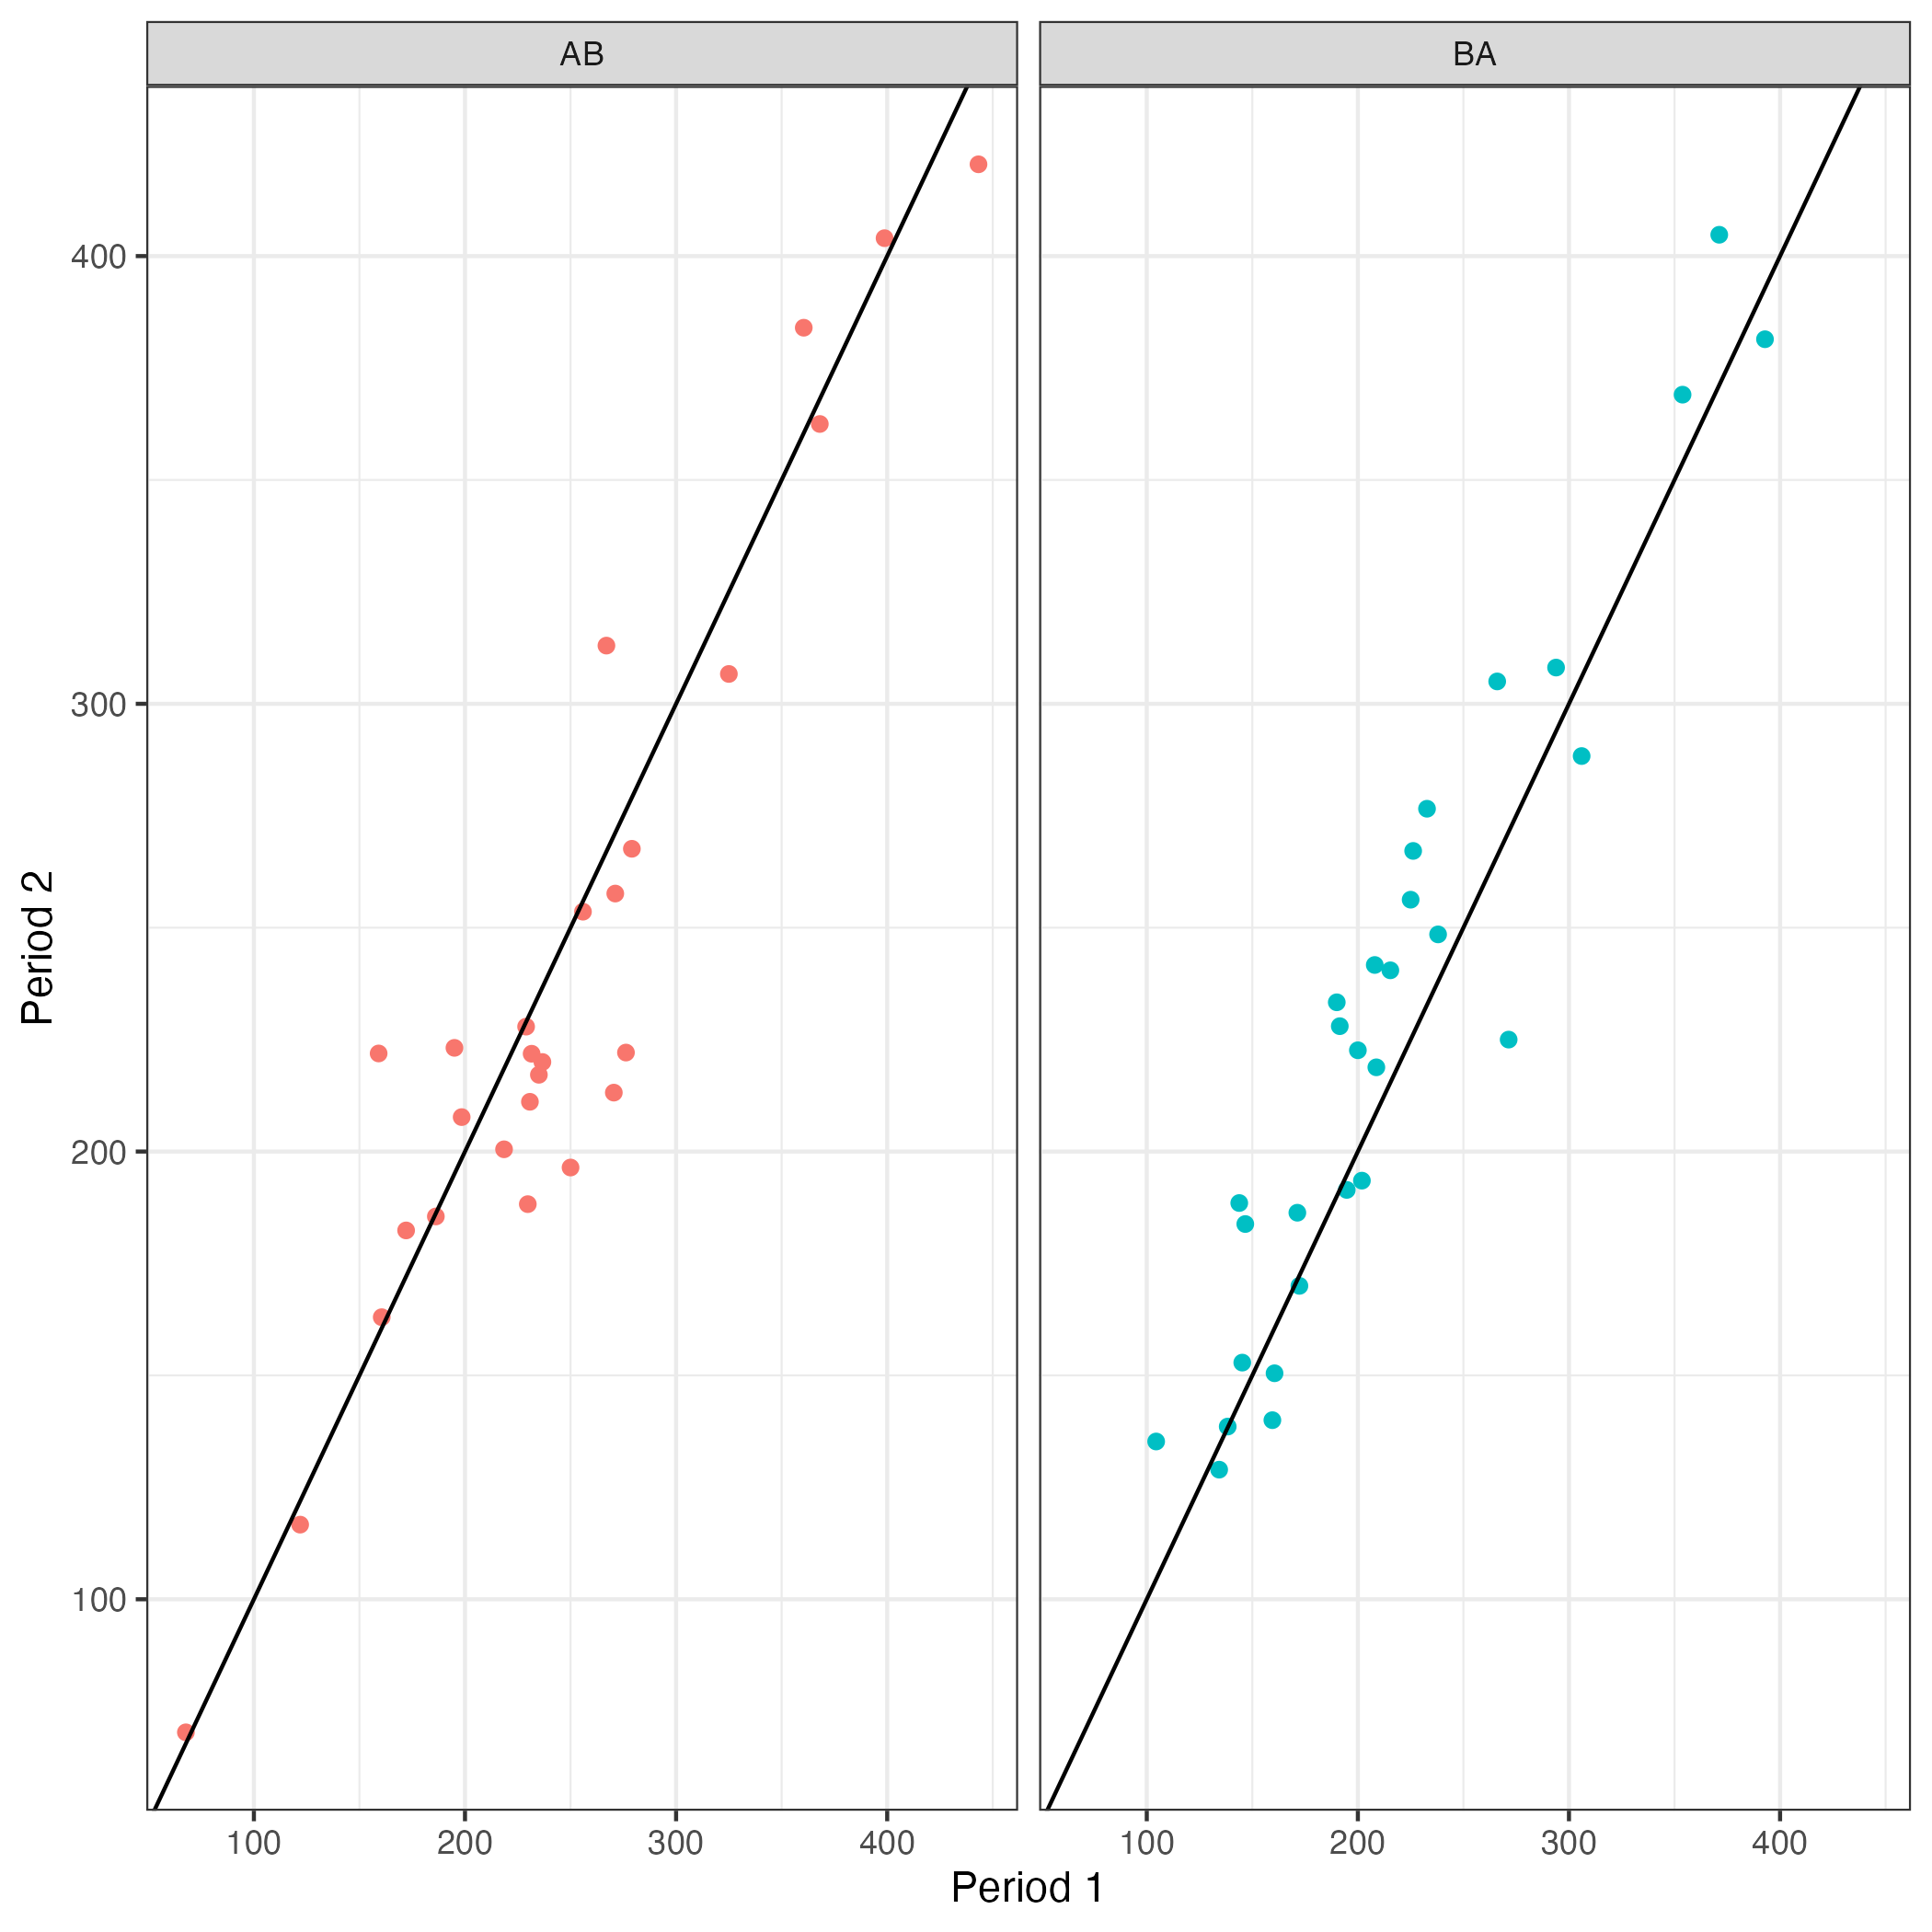
\includegraphics[width=\linewidth]{report/figures/ch2/periodsPlot.png}
    \end{figure}
\end{frame}

\begin{frame}{Period 2 vs Period 1 with Centroids}
    \begin{figure}
        \centering
        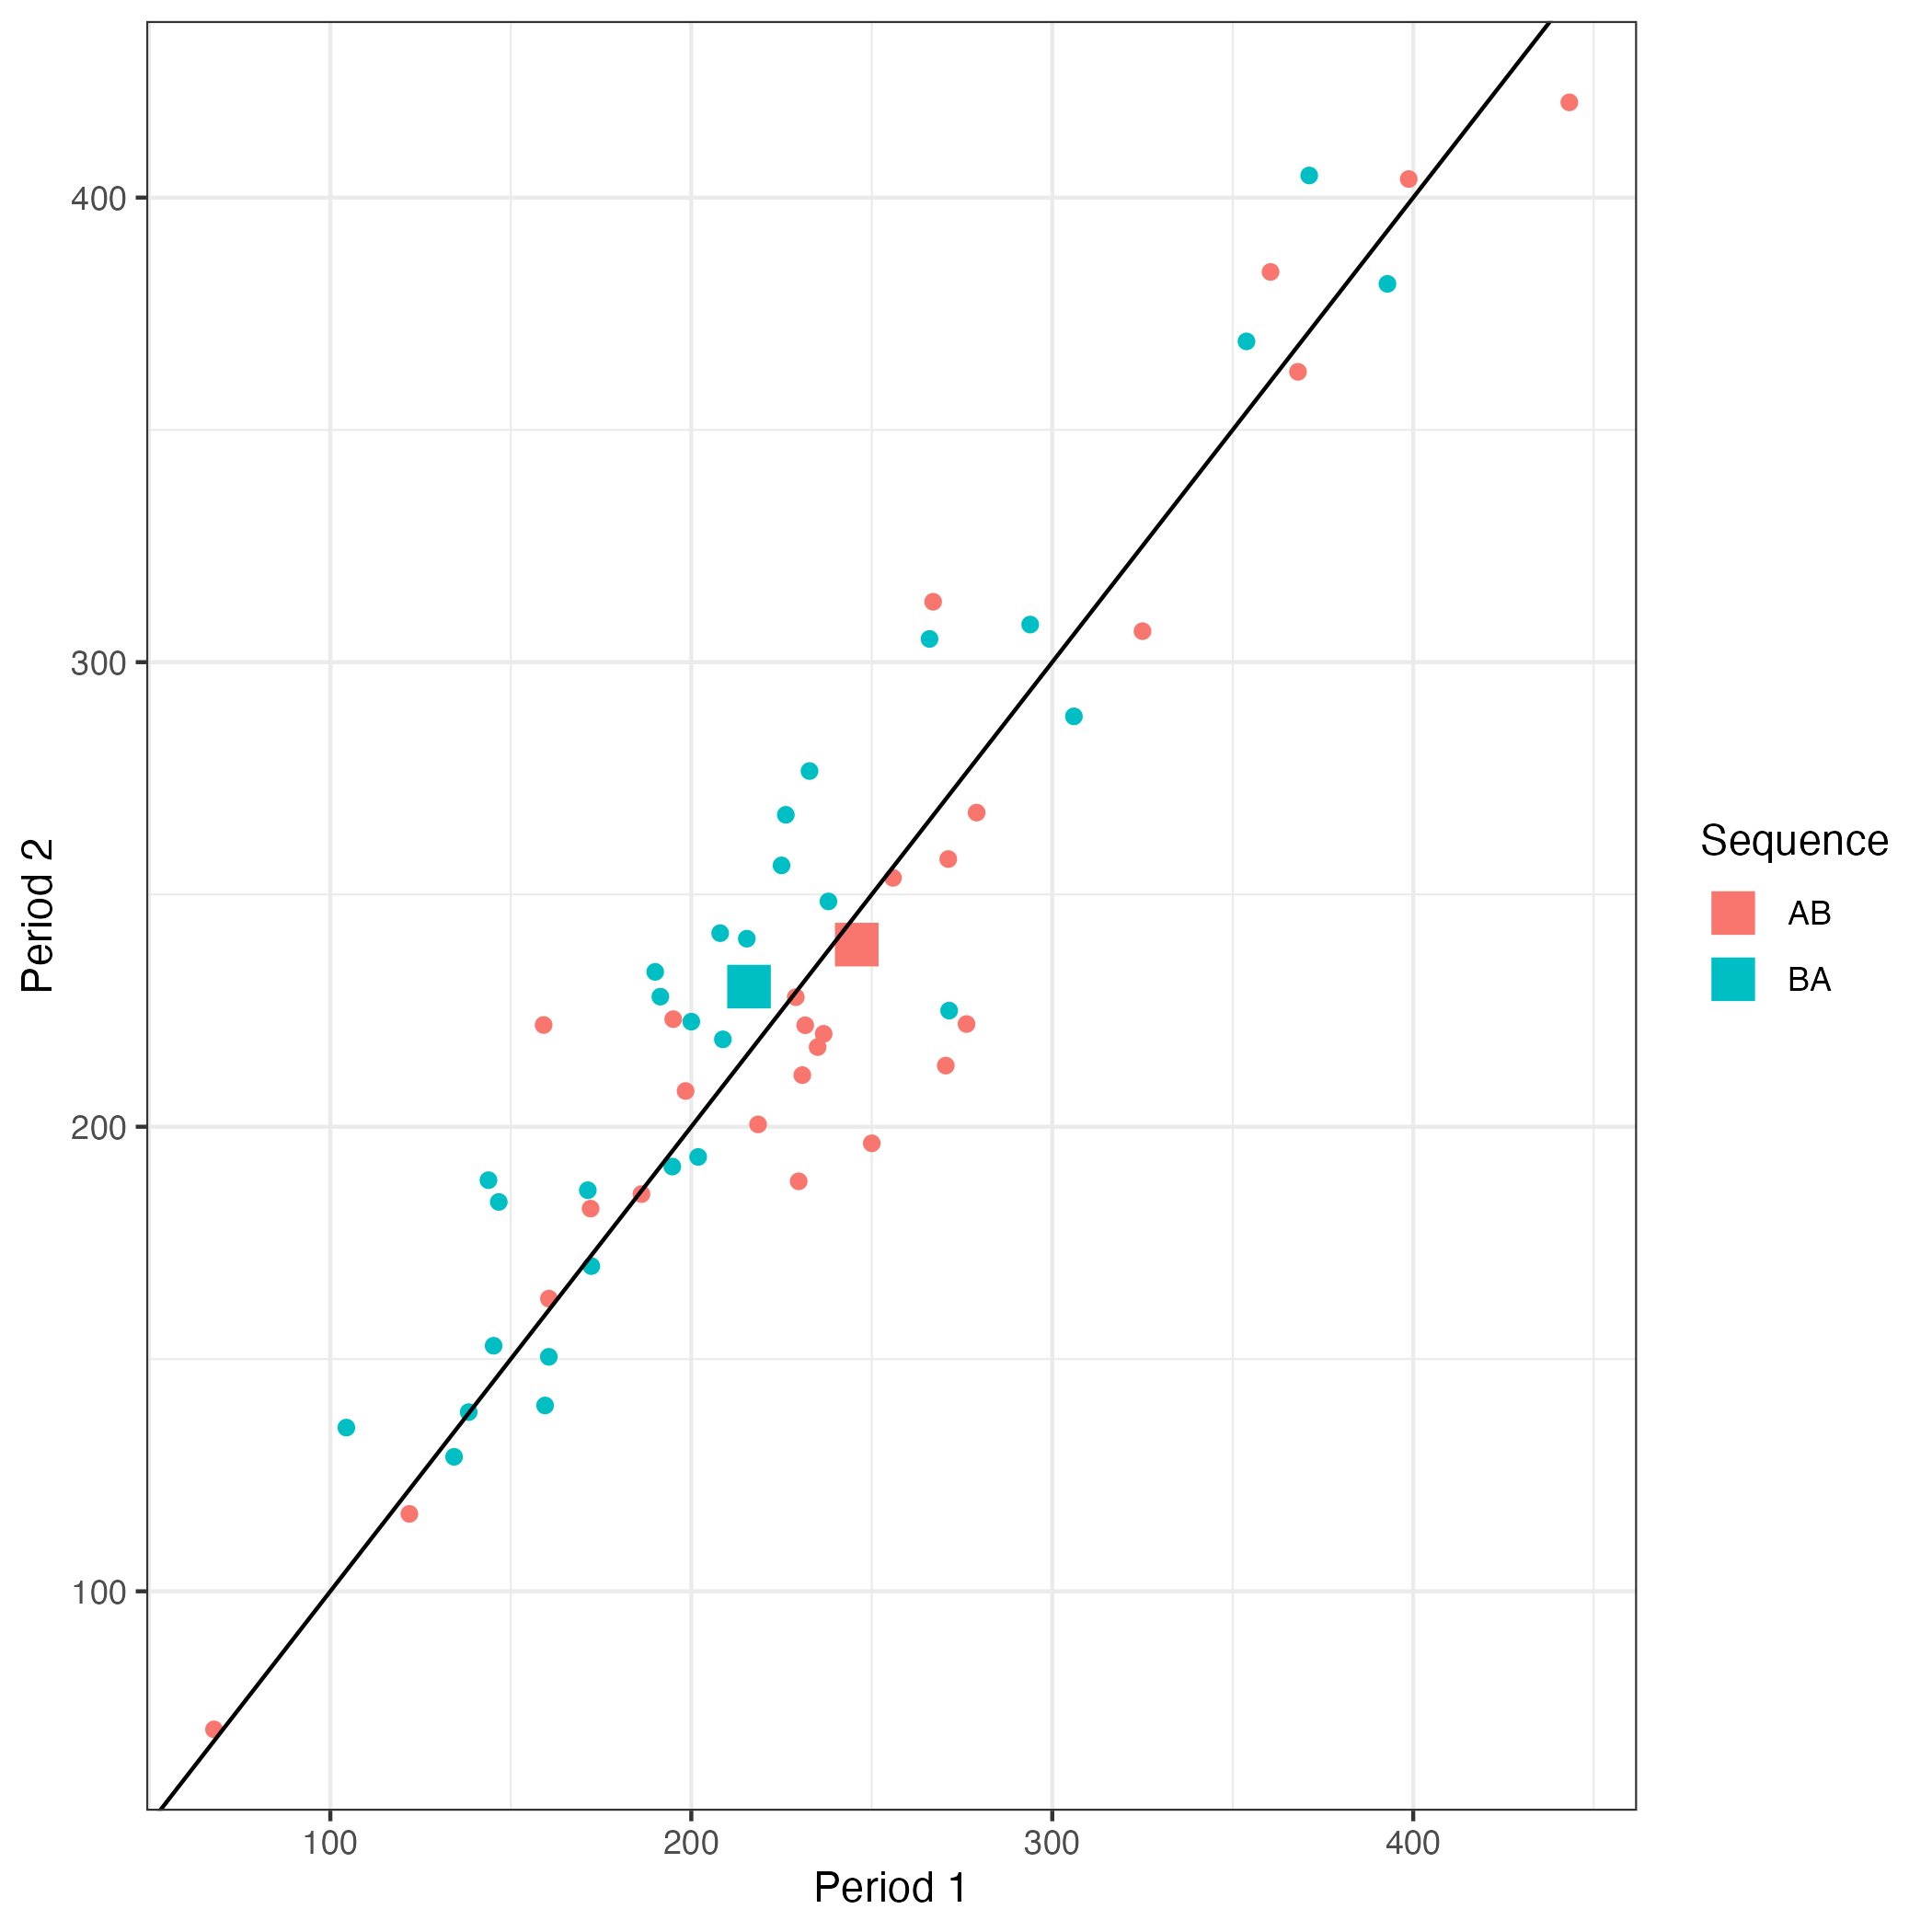
\includegraphics[width=\linewidth]{report/figures/ch2/centroidsPlot.png}
    \end{figure}
    \note[item]{Both groups symmetrical about diagonal line -> no period effect}
    \note[item]{Centroids on opposite sides -> treatment effect}
\end{frame}

\begin{frame}{Groups-by-Periods Plot}
    \begin{figure}
        \centering
        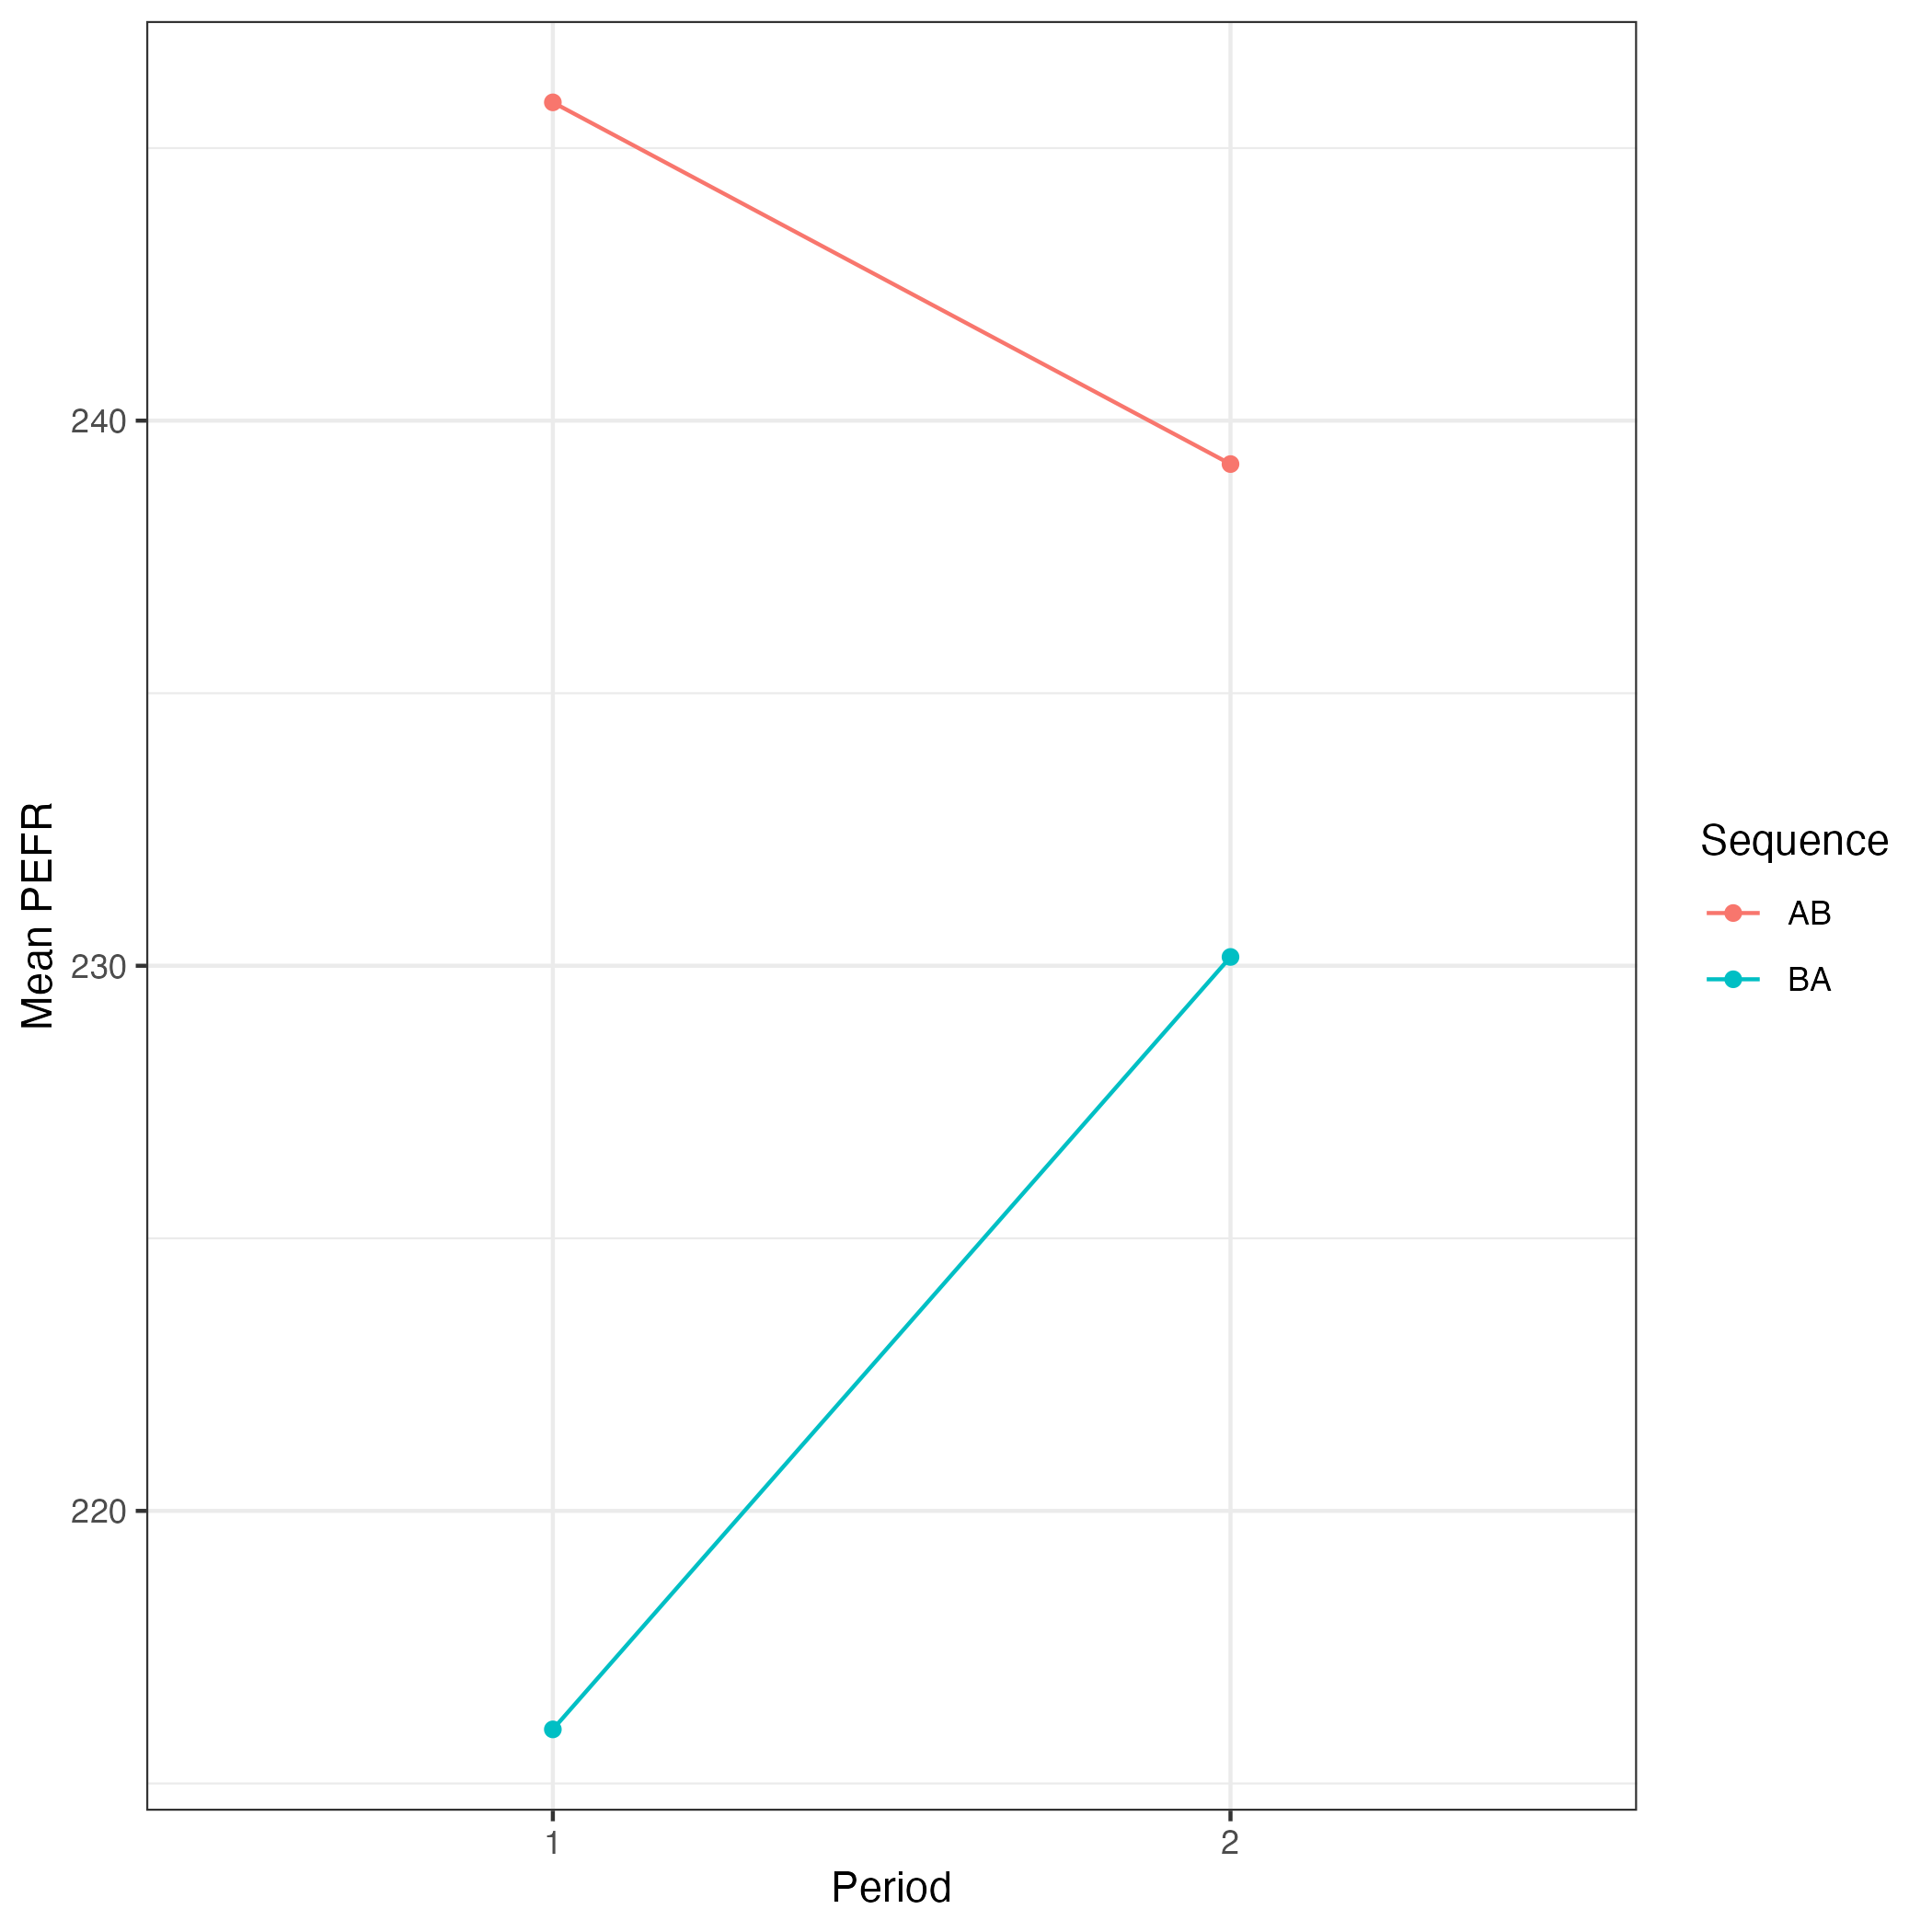
\includegraphics[width=\linewidth]{report/figures/ch2/groupsByPeriodsPlot.png}
    \end{figure}
\end{frame}

\section{Analysis of Cross-Over Trial Data}
\subsection{$t$-Tests}

\begin{frame}{Matched-Pairs $t$-Test}
    \begin{table}

\caption{Matched-Pairs t-Test on COPD Data}
\centering
\begin{tabular}[t]{lllrrrrr}
\toprule
 & Group 1 & Group 2 & n1 & n2 & t-statistic & df & p\\
\midrule
PEFR & A & B & 56 & 56 & 3.081 & 55 & 0.003\\
\bottomrule
\end{tabular}
\end{table}

    \note[item]{Takes advantage of paired structure}
    \note[item]{2-sample t-test equivalent results to PGT}
\end{frame}

\begin{frame}{Assumptions}
    Matched-pairs $t$-test involves two main assumptions:
    \begin{enumerate}
        \item Within-subject differences are independently and randomly distributed around the true treatment effect.
        \item Within-subject differences are distributed approximately normally.
    \end{enumerate}
    Potential assumption violations:
    \begin{itemize}
        \item Period effect
        \item Sequence effect
        \item Period-by-treatment interaction
        \item Carryover
        \item Patient-by-treatment interaction
        \item Patient-by-period interaction
    \end{itemize}
    \note[item]{Period effect: trend over time affecting both groups. Overestimate effect random variation, bias under unbalanced allocation}
    \note[item]{Sequence effect: assume none under successful randomisation.}
    \note[item]{Period-by-treatment: effect of treatment varies by period}
    \note[item]{Patient-by-treatment: effect of treatment varies patient-to-patient}
    \note[item]{Patient-by-period: period effects different for each patient}
    \note[item]{Last two don't affect validity but increase variance.}
\end{frame}

\subsection{Mixed Models}

\begin{frame}{Random-Intercepts Model}
    A random-intercepts mixed model allows us to control for \cite{jones2003design} \cite{mixedmodelsR}:
    \begin{itemize}
        \item Period effect
        \item Sequence effect
        \item Subject-specific effects
        \item Subject-level variables (e.g. sex, age)
    \end{itemize}
    \begin{block}{Mixed Model Equation}
        $Y = \beta_0 + \beta_1 T + \beta_2 P + \beta_3 Se + \beta_{subject} + \epsilon$
    \end{block}
    Three key assumptions \cite{palmieri}:
    \begin{enumerate}
        \item Linearity
        \item Homoscedasticity
        \item Normality of residuals
    \end{enumerate}
    \note[item]{Intercept varies by subject}
\end{frame}

\begin{frame}{Verifying Assumptions: Homoscedasticity}
    \begin{figure}
        \centering
        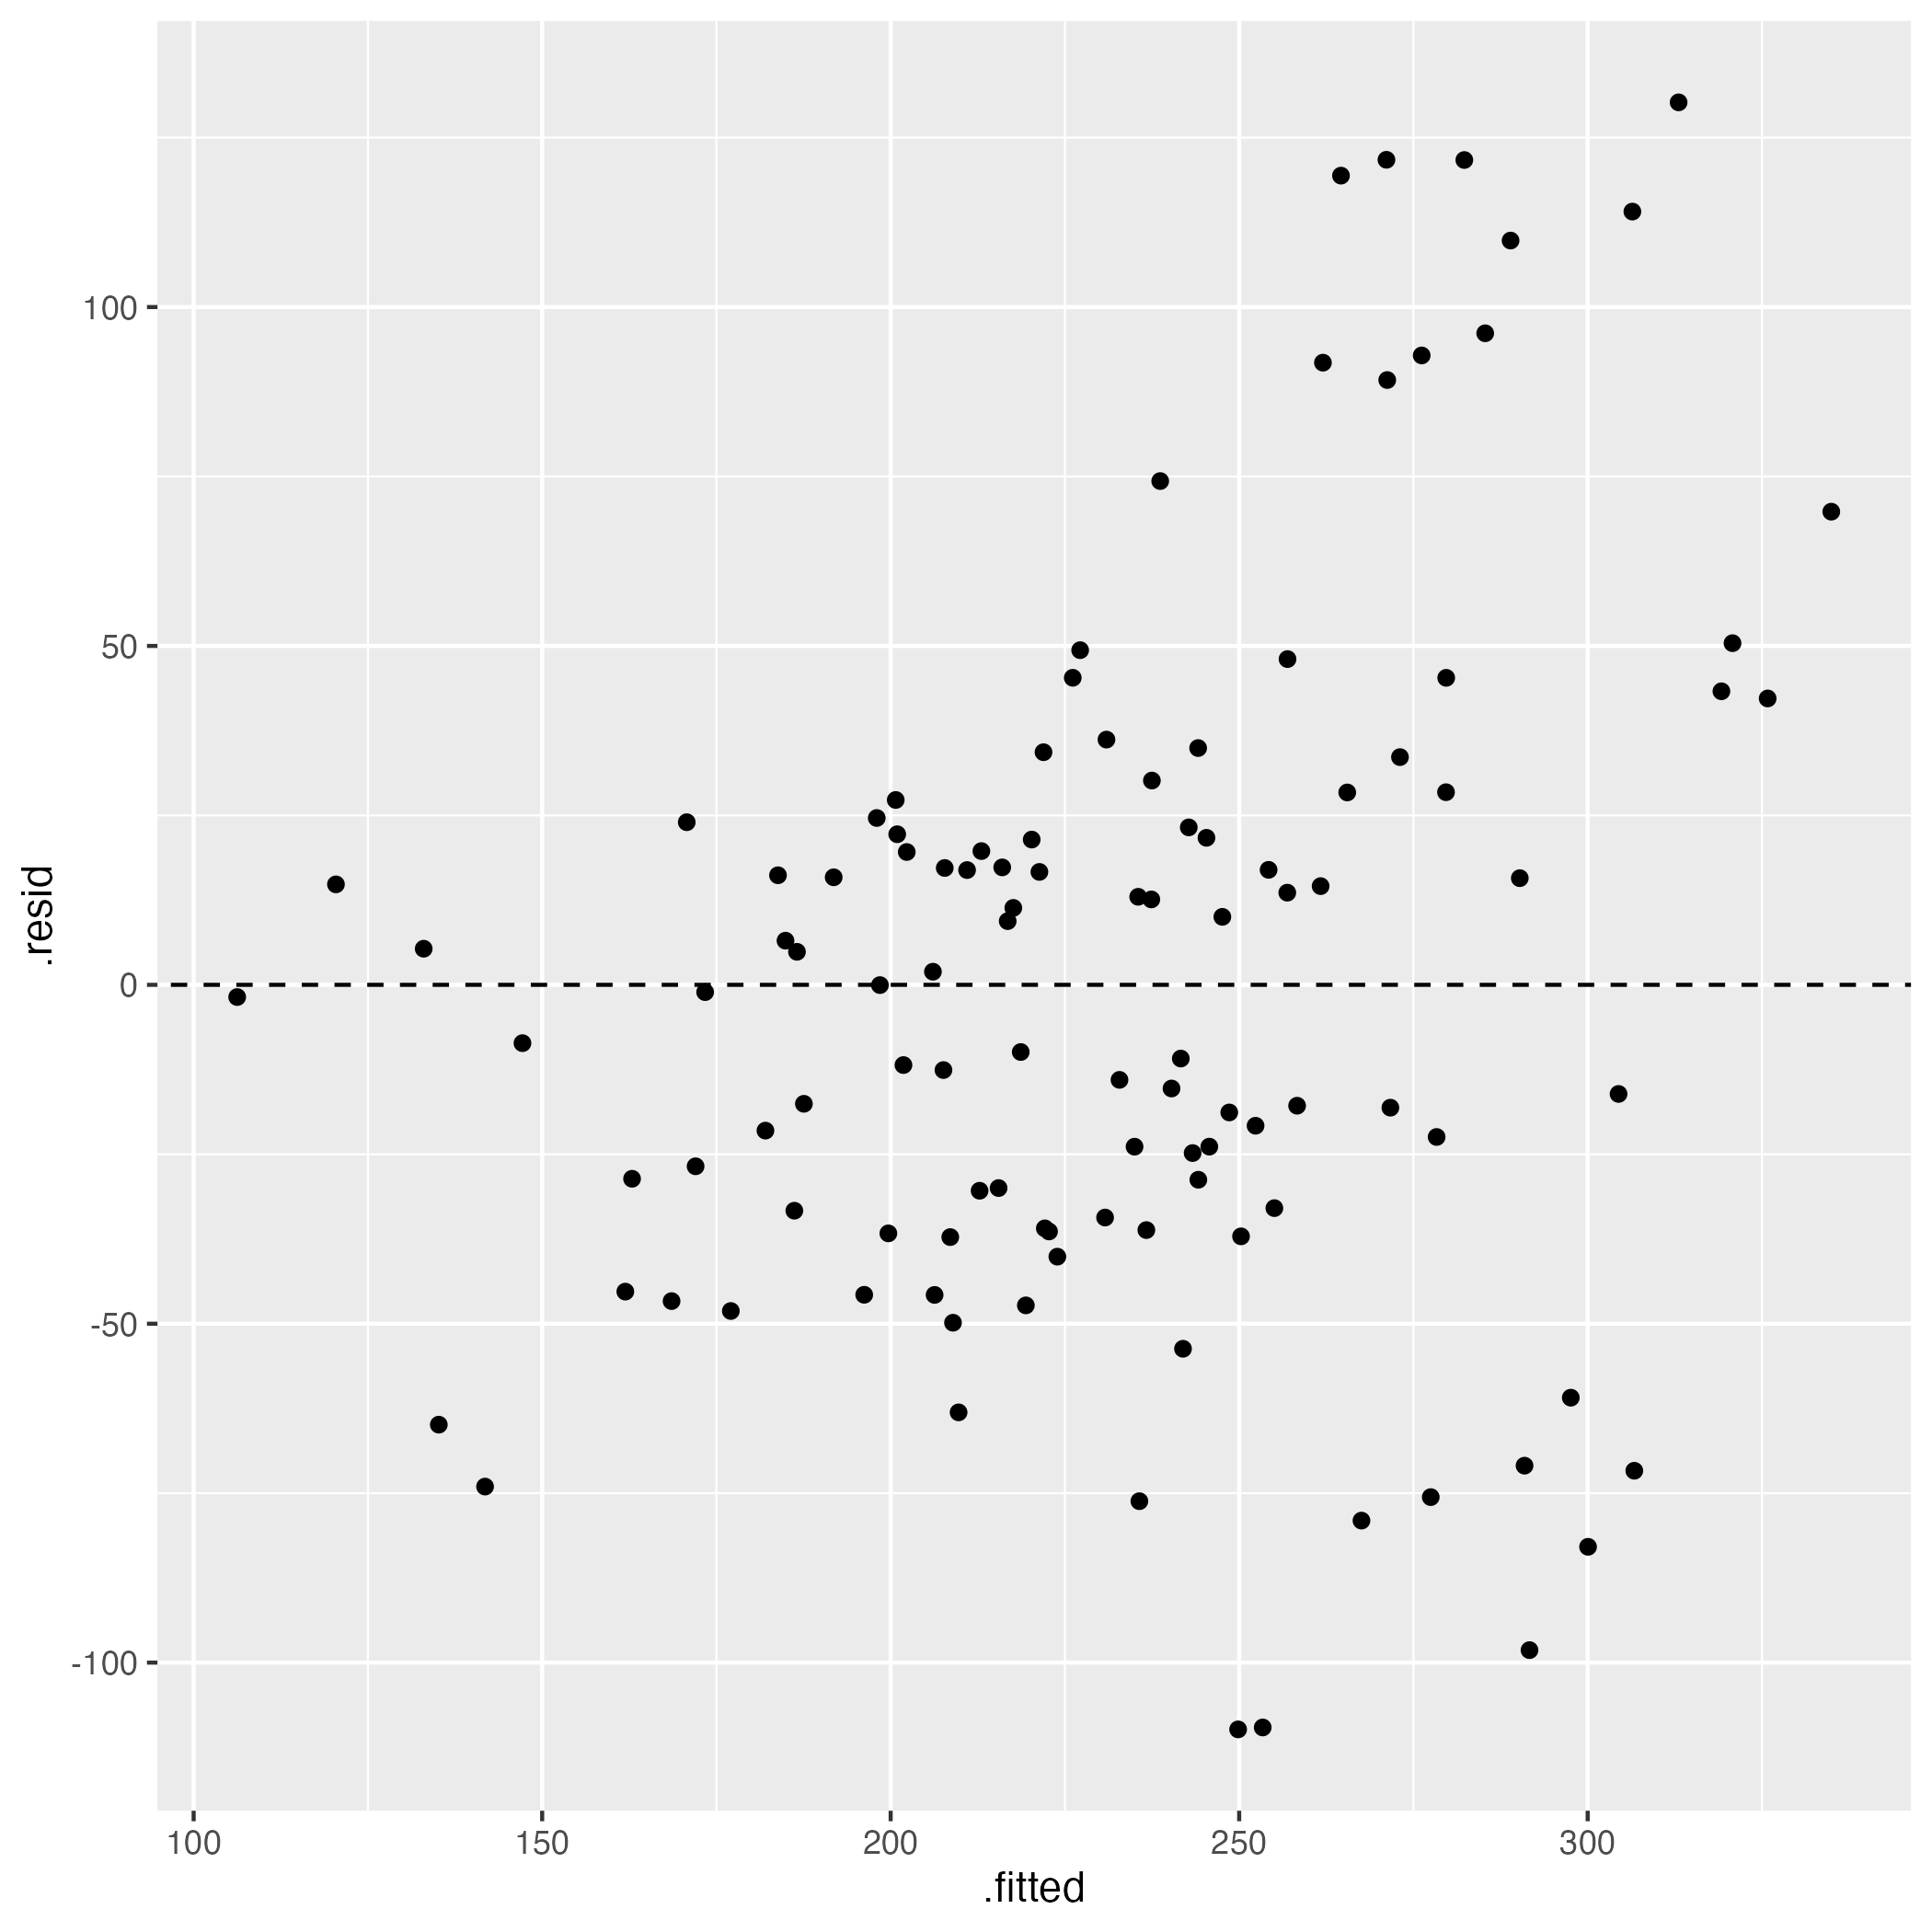
\includegraphics[width=0.75\linewidth]{report/figures/presentation/homoscedasticity.png}
    \end{figure}
\end{frame}

\begin{frame}{Verifying Assumptions: Normality}
    \begin{figure}
        \centering
        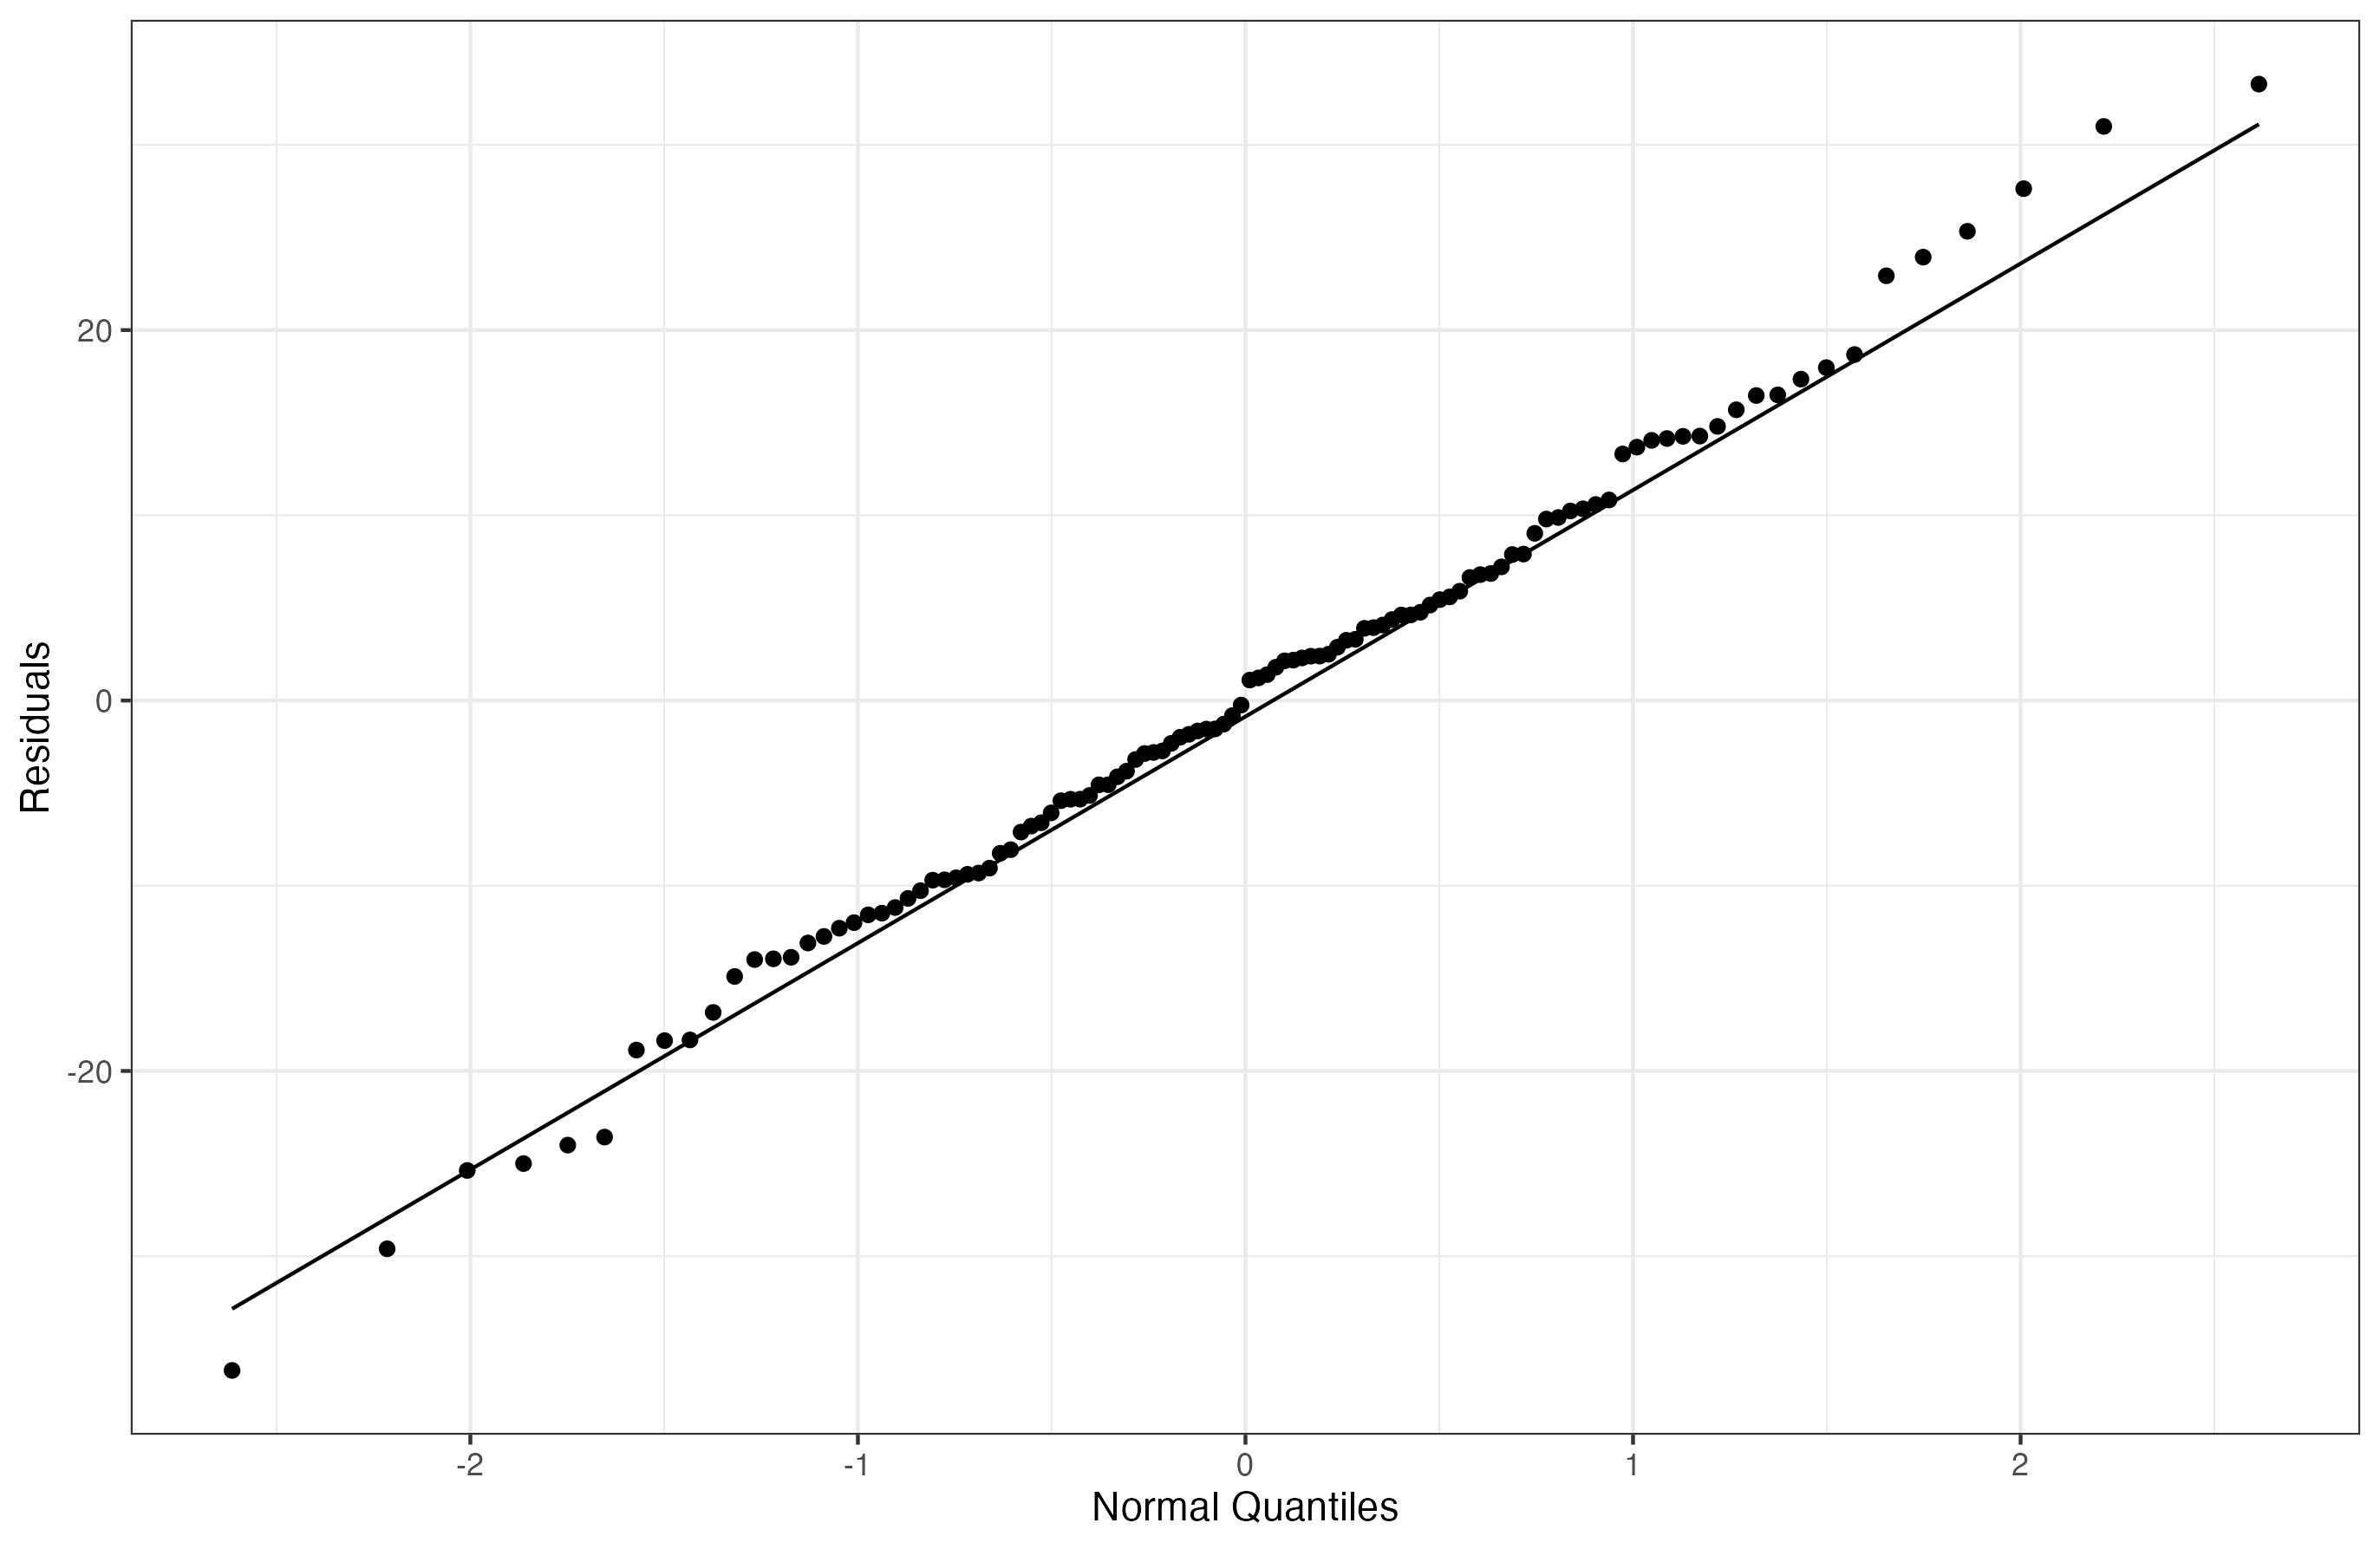
\includegraphics[width=\linewidth]{report/figures/presentation/qqplot.png}
    \end{figure}
\end{frame}

\begin{frame}{Mixed Model Estimates}
    \begin{table}

\caption{Mixed Model Estimates for COPD Data}
\centering
\begin{tabular}[t]{>{}l|rrrrr}
\toprule
 & Estimate & Std. Error & df & t & p\\
\midrule
(Intercept) & 245.84 & 14.96 & 16.43 & 56.99 & $<$0.01\\
TreatB & -10.40 & 3.42 & -3.05 & 54.00 & $<$0.01\\
Period2 & 3.77 & 3.42 & 1.10 & 54.00 & 0.27\\
SequenceBA & -19.44 & 20.50 & -0.95 & 54.00 & 0.35\\
\bottomrule
\end{tabular}
\end{table}

\end{frame}

\begin{frame}{Adjusted Means}
    \begin{table}
\centering
\caption{LS Means for Mixed Model on COPD Data}
\centering
\resizebox{\ifdim\width>\linewidth\linewidth\else\width\fi}{!}{
\begin{tabular}[t]{l>{}l|rrrrr}
\toprule
Sequence & Difference & Adj. Mean & SE & df & Lower CI & Upper CI\\
\midrule
A & . & 238.0 & 10.39 & 56.99 & 212.36 & 263.64\\
B & . & 227.6 & 10.39 & 56.99 & 201.96 & 253.23\\
. & A - B & 10.4 & 3.42 & 54.00 & 1.96 & 18.84\\
\bottomrule
\end{tabular}}
\end{table}

\end{frame}

\subsection{Controlling for Baseline Measurements}

\begin{frame}{Expanded Boxplot}
    \begin{figure}
        \centering
        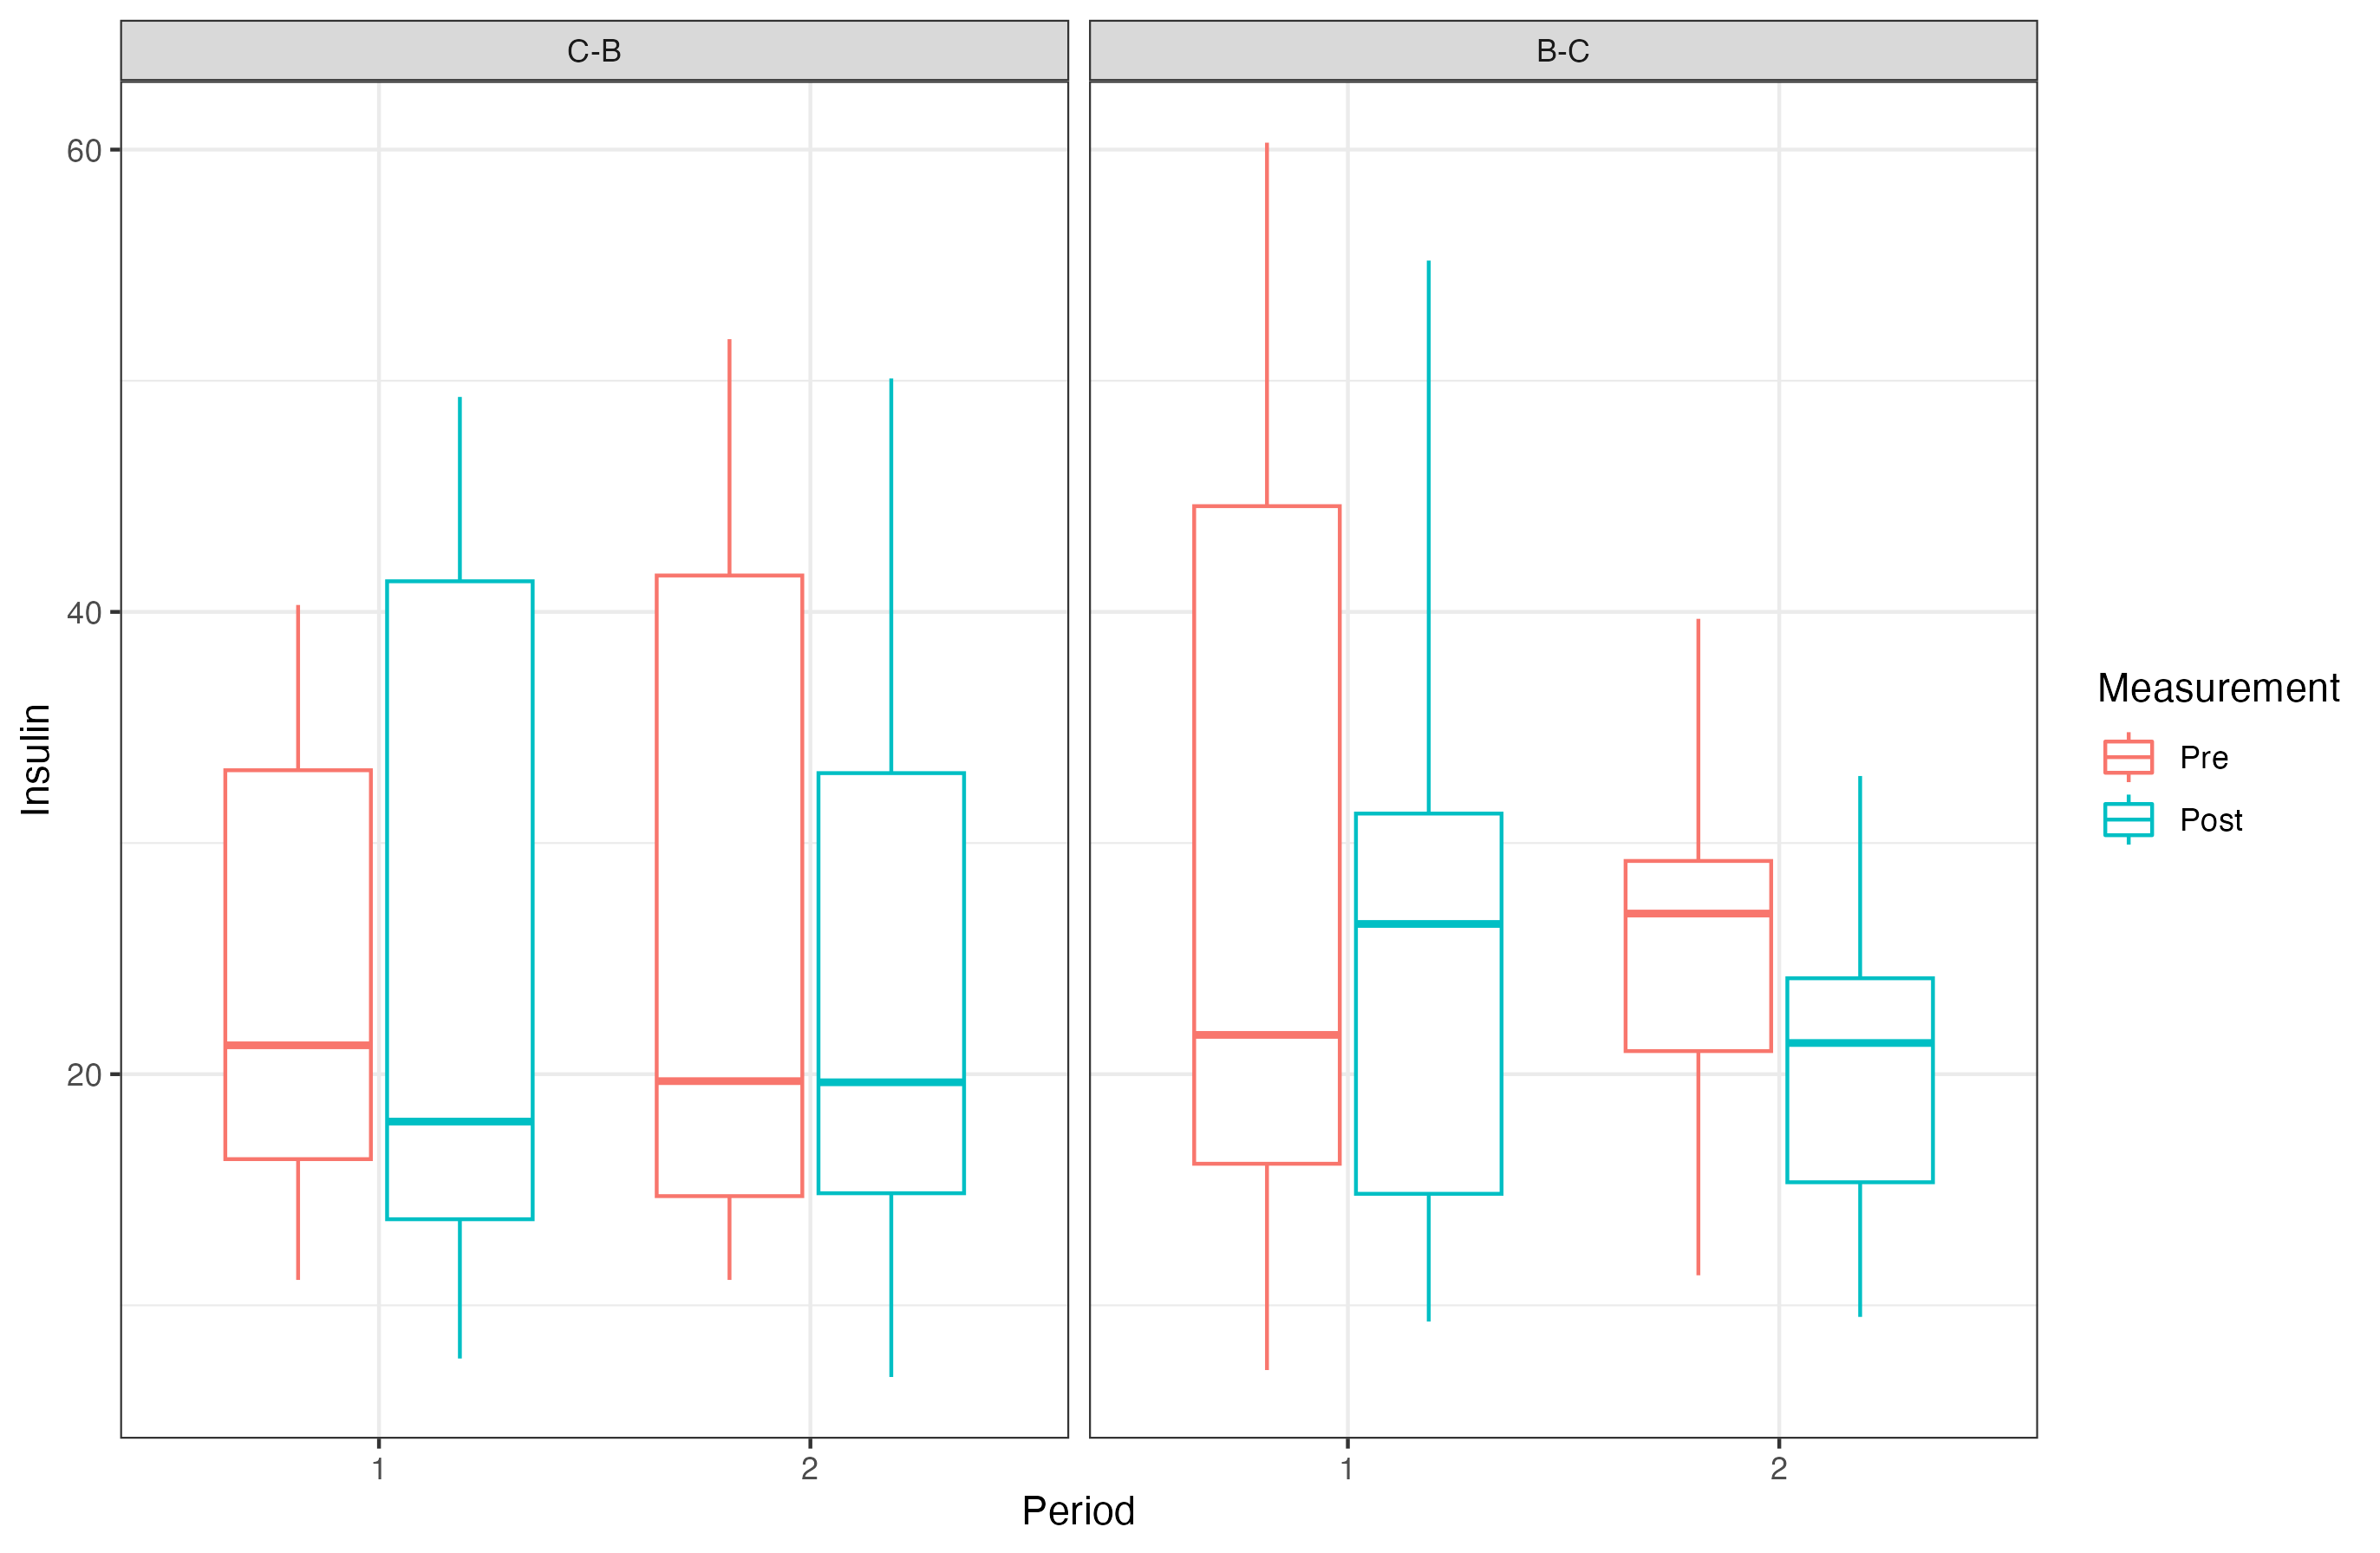
\includegraphics[width=\linewidth]{report/figures/ch3/proteinBoxplot.png}
    \end{figure}
    \note[item]{The trial measured insulin levels after ingesting a protein-based beverage, between beverages with beef- or insect-derived proteins.}
    \note[item]{ 20 subjects  randomised into either C-B or B-C sequence.}
    \note[item]{insulin levels measured just before ingestion (Pre), and 300 minutes after ingestion (Post), resulting in 4 measurements per subject.}
\end{frame}

\begin{frame}{Expanded Summary Table}
    \begin{table}
\centering
\caption{\label{tab:proteinDataSummary}Summary Table for Protein Data (with Baselines)}
\centering
\resizebox{\ifdim\width>\linewidth\linewidth\else\width\fi}{!}{
\begin{tabular}[t]{l>{}r|rrr>{}r|rrrrrrrr}
\toprule
\multicolumn{2}{c}{ } & \multicolumn{4}{c}{Overall} & \multicolumn{4}{c}{Period 1} & \multicolumn{4}{c}{Period 2} \\
\cmidrule(l{3pt}r{3pt}){3-6} \cmidrule(l{3pt}r{3pt}){7-10} \cmidrule(l{3pt}r{3pt}){11-14}
\multicolumn{2}{c}{ } & \multicolumn{2}{c}{Pre} & \multicolumn{2}{c}{Post} & \multicolumn{2}{c}{Pre} & \multicolumn{2}{c}{Post} & \multicolumn{2}{c}{Pre} & \multicolumn{2}{c}{Post} \\
\cmidrule(l{3pt}r{3pt}){3-4} \cmidrule(l{3pt}r{3pt}){5-6} \cmidrule(l{3pt}r{3pt}){7-8} \cmidrule(l{3pt}r{3pt}){9-10} \cmidrule(l{3pt}r{3pt}){11-12} \cmidrule(l{3pt}r{3pt}){13-14}
Sequence & Subject & Mean & SD & Mean & SD & Mean & SD & Mean & SD & Mean & SD & Mean & SD\\
\midrule
C-B & 10 & 25.71 & 13.53 & 24.55 & 14.43 & 24.03 & 10.70 & 25.13 & 16.07 & 27.39 & 16.31 & 23.97 & 13.45\\
B-C & 10 & 27.91 & 14.39 & 23.12 & 11.11 & 29.73 & 18.94 & 25.84 & 13.83 & 26.10 & 8.44 & 20.40 & 7.27\\
\midrule\\
Total & 20 & 26.81 & 13.83 & 23.84 & 12.74 & 26.88 & 15.25 & 25.48 & 14.60 & 26.75 & 12.66 & 22.18 & 10.68\\
\bottomrule
\end{tabular}}
\end{table}

\end{frame}

\begin{frame}{Adjusting for Baseline Values}
    \begin{itemize}
        \item ANCOVA incorporates baseline measurements as a covariate in pre-post designs.
        \item Cross-over designs requires measurements for each subject prior to each treatment period to incorporate baselines.
        \item Most efficient method is to include \textit{within-subject difference in baselines} as an interaction with the period effect \cite{mehrotra2014}.
    \end{itemize}
    \begin{block}{Mixed Model with Baselines}
        $Y = \beta_0 + \beta_1 T + \beta_2 P \cdot X_{diff} + \beta_3 P + \beta_4 X_{diff} + \beta_5 Se + \beta_{subject} + \epsilon$
    \end{block}
    \note[item]{4 total measurements per subject}
\end{frame}

\begin{frame}{Mixed Model Estimates with Baselines}
    \begin{table}[b]

\caption{\label{tab:proteinDataEstimates}Mixed Model Estimates with Baseline Interaction}
\centering
\begin{tabular}[t]{>{}l|rrrrr}
\toprule
 & Estimate & Std. Error & df & t & p-value\\
\midrule
(Intercept) & 25.30 & 4.23 & 5.97 & 20.55 & 0.00\\
TreatmentBEEF & 0.71 & 1.90 & 0.37 & 17.00 & 0.71\\
Period2 & -3.24 & 1.81 & -1.79 & 17.00 & 0.09\\
Pre\_diff & 0.05 & 0.26 & 0.19 & 20.55 & 0.85\\
SequenceB-C & -0.35 & 5.84 & -0.06 & 17.00 & 0.95\\
Period2:Pre\_diff & -0.41 & 0.16 & -2.50 & 17.00 & 0.02\\
\bottomrule
\end{tabular}
\end{table}

    \notep[item]{Can also calculate LS means}
\end{frame}

\begin{frame}{Bibliography}
    \bibliography{report/references}
    \bibliographystyle{ieeetr}
\end{frame}

\end{document}